\documentclass[11pt,a3paper,landscape]{article}
\usepackage[utf8]{inputenc}
\usepackage[T1]{fontenc}
\usepackage[paperwidth=42cm,paperheight=29.7cm,margin=0.8cm]{geometry}
\usepackage{tikz}
\usepackage{graphicx}
\usetikzlibrary{arrows.meta,positioning,fit,backgrounds,calc}

\definecolor{pastelRuntime}{RGB}{220,234,252}
\definecolor{pastelApi}{RGB}{226,245,230}
\definecolor{pastelServices}{RGB}{255,239,219}
\definecolor{pastelSchemas}{RGB}{236,230,252}
\definecolor{pastelExceptions}{RGB}{255,243,214}

\begin{document}
\pagestyle{empty}

\begin{center}
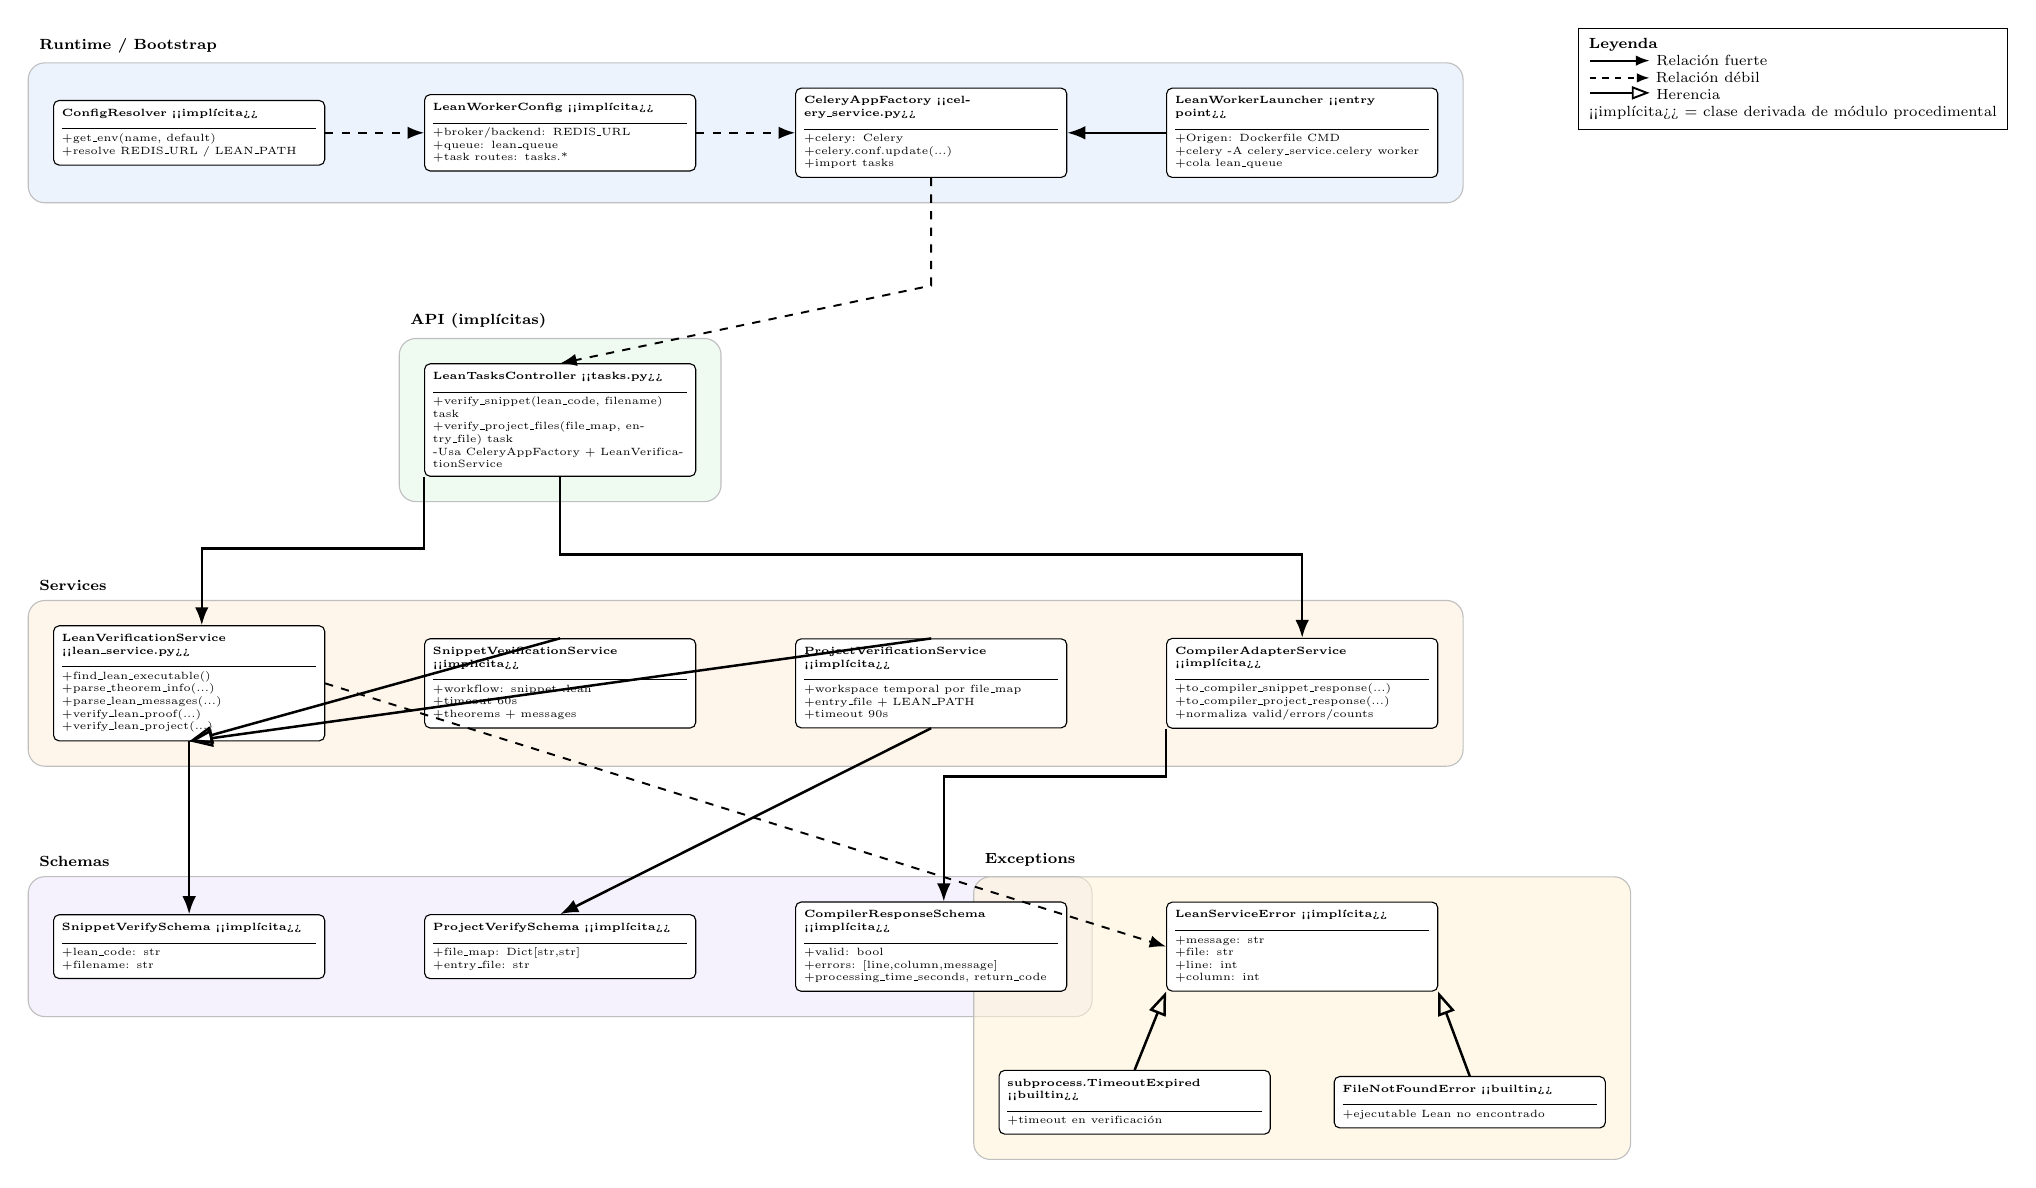
\begin{tikzpicture}[
  scale=0.76,
  transform shape,
  x=1cm,
  y=1cm,
  classbox/.style={
    draw,
    rounded corners=2pt,
    align=left,
    font=\tiny,
    text width=4.25cm,
    inner sep=4pt,
    fill=white
  },
  sectionbox/.style={draw=black!25, line width=0.4pt, rounded corners=6pt, inner sep=9pt, fill opacity=0.55},
  strong/.style={-{Latex[length=2.3mm]}, line width=0.9pt},
  weak/.style={-{Latex[length=2.1mm]}, line width=0.7pt, dashed},
  inherit/.style={-{Triangle[open,length=3mm,width=2.2mm]}, line width=0.9pt},
  rel/.style={font=\tiny, fill=white, inner sep=1pt}
]

% =========================
% Runtime / Bootstrap
% =========================
\node[classbox] (configResolver) at (0,12) {
\textbf{ConfigResolver <<implícita>>}\\
\rule{\linewidth}{0.2pt}\\
+get\_env(name, default)\\
+resolve REDIS\_URL / LEAN\_PATH
};

\node[classbox] (workerConfig) at (6.2,12) {
\textbf{LeanWorkerConfig <<implícita>>}\\
\rule{\linewidth}{0.2pt}\\
+broker/backend: REDIS\_URL\\
+queue: lean\_queue\\
+task routes: tasks.*
};

\node[classbox] (celeryFactory) at (12.4,12) {
\textbf{CeleryAppFactory <<celery\_service.py>>}\\
\rule{\linewidth}{0.2pt}\\
+celery: Celery\\
+celery.conf.update(...)\\
+import tasks
};

\node[classbox] (workerLauncher) at (18.6,12) {
\textbf{LeanWorkerLauncher <<entry point>>}\\
\rule{\linewidth}{0.2pt}\\
+Origen: Dockerfile CMD\\
+celery -A celery\_service.celery worker\\
+cola lean\_queue
};

% =========================
% API Layer (procedural -> implicit classes)
% =========================
\node[classbox] (tasksController) at (6.2,7.2) {
\textbf{LeanTasksController <<tasks.py>>}\\
\rule{\linewidth}{0.2pt}\\
+verify\_snippet(lean\_code, filename) {task}\\
+verify\_project\_files(file\_map, entry\_file) {task}\\
-Usa CeleryAppFactory + LeanVerificationService
};

% =========================
% Services
% =========================
\node[classbox] (leanService) at (0,2.8) {
\textbf{LeanVerificationService <<lean\_service.py>>}\\
\rule{\linewidth}{0.2pt}\\
+find\_lean\_executable()\\
+parse\_theorem\_info(...)\\
+parse\_lean\_messages(...)\\
+verify\_lean\_proof(...)\\
+verify\_lean\_project(...)
};

\node[classbox] (snippetService) at (6.2,2.8) {
\textbf{SnippetVerificationService <<implícita>>}\\
\rule{\linewidth}{0.2pt}\\
+workflow: snippet .lean\\
+timeout 60s\\
+theorems + messages
};

\node[classbox] (projectService) at (12.4,2.8) {
\textbf{ProjectVerificationService <<implícita>>}\\
\rule{\linewidth}{0.2pt}\\
+workspace temporal por file\_map\\
+entry\_file + LEAN\_PATH\\
+timeout 90s
};

\node[classbox] (compilerAdapter) at (18.6,2.8) {
\textbf{CompilerAdapterService <<implícita>>}\\
\rule{\linewidth}{0.2pt}\\
+to\_compiler\_snippet\_response(...)\\
+to\_compiler\_project\_response(...)\\
+normaliza valid/errors/counts
};

% =========================
% Schemas
% =========================
\node[classbox] (snippetSchema) at (0,-1.6) {
\textbf{SnippetVerifySchema <<implícita>>}\\
\rule{\linewidth}{0.2pt}\\
+lean\_code: str\\
+filename: str
};

\node[classbox] (projectSchema) at (6.2,-1.6) {
\textbf{ProjectVerifySchema <<implícita>>}\\
\rule{\linewidth}{0.2pt}\\
+file\_map: Dict[str,str]\\
+entry\_file: str
};

\node[classbox] (compilerResponseSchema) at (12.4,-1.6) {
\textbf{CompilerResponseSchema <<implícita>>}\\
\rule{\linewidth}{0.2pt}\\
+valid: bool\\
+errors: [{line,column,message}]\\
+processing\_time\_seconds, return\_code
};

% =========================
% Exceptions
% =========================
\node[classbox] (leanServiceErr) at (18.6,-1.6) {
\textbf{LeanServiceError <<implícita>>}\\
\rule{\linewidth}{0.2pt}\\
+message: str\\
+file: str\\
+line: int\\
+column: int
};

\node[classbox] (timeoutErr) at (15.8,-4.2) {
\textbf{subprocess.TimeoutExpired <<builtin>>}\\
\rule{\linewidth}{0.2pt}\\
+timeout en verificación
};

\node[classbox] (fileNotFoundErr) at (21.4,-4.2) {
\textbf{FileNotFoundError <<builtin>>}\\
\rule{\linewidth}{0.2pt}\\
+ejecutable Lean no encontrado
};

% =========================
% Grouping boxes
% =========================
\begin{scope}[on background layer]
  \node[sectionbox, fill=pastelRuntime, fit=(configResolver)(workerLauncher)] (bgRuntime) {};
  \node[sectionbox, fill=pastelApi, fit=(tasksController)] (bgApi) {};
  \node[sectionbox, fill=pastelServices, fit=(leanService)(compilerAdapter)] (bgServices) {};
  \node[sectionbox, fill=pastelSchemas, fit=(snippetSchema)(compilerResponseSchema)] (bgSchemas) {};
  \node[sectionbox, fill=pastelExceptions, fit=(leanServiceErr)(timeoutErr)(fileNotFoundErr)] (bgExceptions) {};

  \node[font=\scriptsize\bfseries, anchor=south west] at ($(bgRuntime.north west)+(2pt,1pt)$) {Runtime / Bootstrap};
  \node[font=\scriptsize\bfseries, anchor=south west] at ($(bgApi.north west)+(2pt,1pt)$) {API (implícitas)};
  \node[font=\scriptsize\bfseries, anchor=south west] at ($(bgServices.north west)+(2pt,1pt)$) {Services};
  \node[font=\scriptsize\bfseries, anchor=south west] at ($(bgSchemas.north west)+(2pt,1pt)$) {Schemas};
  \node[font=\scriptsize\bfseries, anchor=south west] at ($(bgExceptions.north west)+(2pt,1pt)$) {Exceptions};
\end{scope}

% =========================
% Relations
% =========================
\draw[weak] (configResolver.east) -- (workerConfig.west);
\draw[weak] (workerConfig.east) -- (celeryFactory.west);
\draw[strong] (workerLauncher.west) -- (celeryFactory.east);

\draw[weak] ([xshift=0pt]celeryFactory.south) -- ++(0,-1.8) -- ([xshift=0pt]tasksController.north);

\draw[strong] (tasksController.south west) -- ++(0,-1.2) -| ([xshift=6pt]leanService.north);
\draw[strong] (tasksController.south) -- ++(0,-1.3) -| ([xshift=0pt]compilerAdapter.north);

\draw[inherit] (snippetService.north) -- (leanService.south);
\draw[inherit] (projectService.north) -- (leanService.south);

\draw[strong] (leanService.south) -- (snippetSchema.north);
\draw[strong] (projectService.south) -- (projectSchema.north);
\draw[strong] (compilerAdapter.south west) -- ++(0,-0.8) -| ([xshift=6pt]compilerResponseSchema.north);

\draw[weak] (leanService.east) -- (leanServiceErr.west);
\draw[inherit] (timeoutErr.north) -- (leanServiceErr.south west);
\draw[inherit] (fileNotFoundErr.north) -- (leanServiceErr.south east);

% Legend
\node[draw, align=left, font=\scriptsize, inner sep=5pt, fill=white] at (26.8,12.9) (legend) {
\textbf{Leyenda}\\
\tikz{\draw[strong] (0,0)--(1.0,0);} Relación fuerte\\
\tikz{\draw[weak] (0,0)--(1.0,0);} Relación débil\\
\tikz{\draw[inherit] (0,0)--(1.0,0);} Herencia\\
<<implícita>> = clase derivada de módulo procedimental
};

\end{tikzpicture}
\end{center}

\end{document}
